\chapter{Constructing the TreeFam} \label{chap:treefam}

Genes are related in the context of evolution.
To transfer functional annotations across different species
and to study the principle of gene evolution, it is important
to untangle the relationships between the genes in a gene family. The best
way to achieve this is to reconstruct a phylogenetic tree, which
not only presents most of evolutionary details, but also provides
the basis for further studies such as ortholog inference and
gene annotation. TreeFam~\cite{li06} (Tree families database)\index{TreeFam}
is a database of phylogenetic trees of gene families. It aims
to develop a curated resource that presents the accurate evolutionary
history of all metazoan animal gene families, as well as various inference 
based on phylogenetic trees.

In this chapter, we will introduce TreeFam database, its contents,
structures, and pipelines that are used to construct TreeFam.
As detailed procedures used by TreeFam-1.x have already been described
in our paper, we will put more emphasis on the difference between
release 1.x and 2.0 when presenting the whole pipelines.

\section{Overview of TreeFam}
\subsection{What is TreeFam?}
TreeFam is first a protein classification database. It aims to classify
genes into families, and assign a name to each family and significant
subfamily. Distinguished from most of other similar databases like
KOG~\cite{tatusov03}, PANTHER~\cite{mi05} and SYSTERS~\cite{meinel05}, which defines families according to the degree
of similarities between family members, TreeFam aims to define a gene
family as a group of genes that descended from a single gene in
the last common ancestor of all metazoan animal, or that first appeared in metazoan animals.
Evolutionary rates, reflected by similarity scores, may vary greatly in different
groups of genes. Families defined by similarity based methods
will be inevitably sensitive to the threshold that is used at clustering stage,
and also lack biological meaning.
In contrast, TreeFam will not suffer from this problem. As is pointed by
PhIGs~\cite{dehal05}, which is one of the basis of TreeFam, families defined in the phylogenetic way
are not sensitive to similarity threshold, and therefore more
robust and meaningful from the evolutionary angle.

Secondly, TreeFam is an ortholog database\index{ortholog!ortholog database}. It infers orthologs and paralogs from
the phylogenetic tree of a gene family. Traditionally, orthologs are inferred from
pairwise alignment between two species with a little help of synteny for close related species. Most of ortholog database at present are
based on this method, including NCBI HomoloGene~\cite{wheeler05},
Ensembl-compara~\cite{hubbard05}, OrthoMCL~\cite{li03}, and Inparanoid~\cite{o'brien05}.
Although these databases provide useful information about ortholog assignment,
they might fall short when gene loss interferes. In the absence of
genes from third-part species, pairwise method might overlook the existence
of duplications and therefore overestimate orthologs.
Furthermore, their inference between different pairs of species might be inconsistent.
For example, assume gene $g_1$ is a 1:1 ortholog of $g_2$, and $g_2$ is a 1:1 ortholog of $g_3$. Then
$g_1$ should also be one-to-one orthologous to $g_3$ in theory. But in pairwise framework, it is possible
that $g_1$ is not an ortholog of $g_3$. This is because the three pairs, $(g_1,g_2)$, $(g_2,g_3)$
and $(g_3,g_1)$, are processed separately. It is not required that they should be consistent.
In contrast, Tree-based method, considering genes from multiple species as a whole, will not suffer from these problems.
It is also more intuitive and informative in comparison with pairwise method.
To the best of our knowledge, only HOGENOM~\cite{dufayard05} has inferred orthologs from
phylogenetic trees.

Finally, TreeFam is a curated database. Evolution diverges in different gene families
and also in different lineages. To automatically reconstruct reliable phylogenetic trees is always
one of the most challenging topics in the area of bioinformatics. This is why biologists have to reduce to
pairwise methods even when they know the advantage of tree-based methods. Although in TreeFam we have developed new algorithms to improve
the accuracy, automatic process is not comparable to human curation. Only
human being can successfully integrate information from various resources;
only human being can endow a tree with biological meaning. TreeFam is unique because
it incorporates human curation.

\subsection{Basic Structures of TreeFam}
The basic structure of TreeFam resembles that of Pfam~\cite{bateman04}, a curated resource for
protein domains. Like Pfam, TreeFam is also a biparted database: part A
that consists of curated tree families, and part B that consists of automatically
generated families. Each part also comprises of two types of sequences:
seed that come from either manual curation (for TreeFam-A) or PhIGs clusters (for TreeFam-B),
and full sequences that are expanded from seeds. Figure~\ref{fig:flowchart}(A) presents the overall
relations between these concepts. Detailed pipelines will be explained in
following sections.

\begin{figure}[!hb]
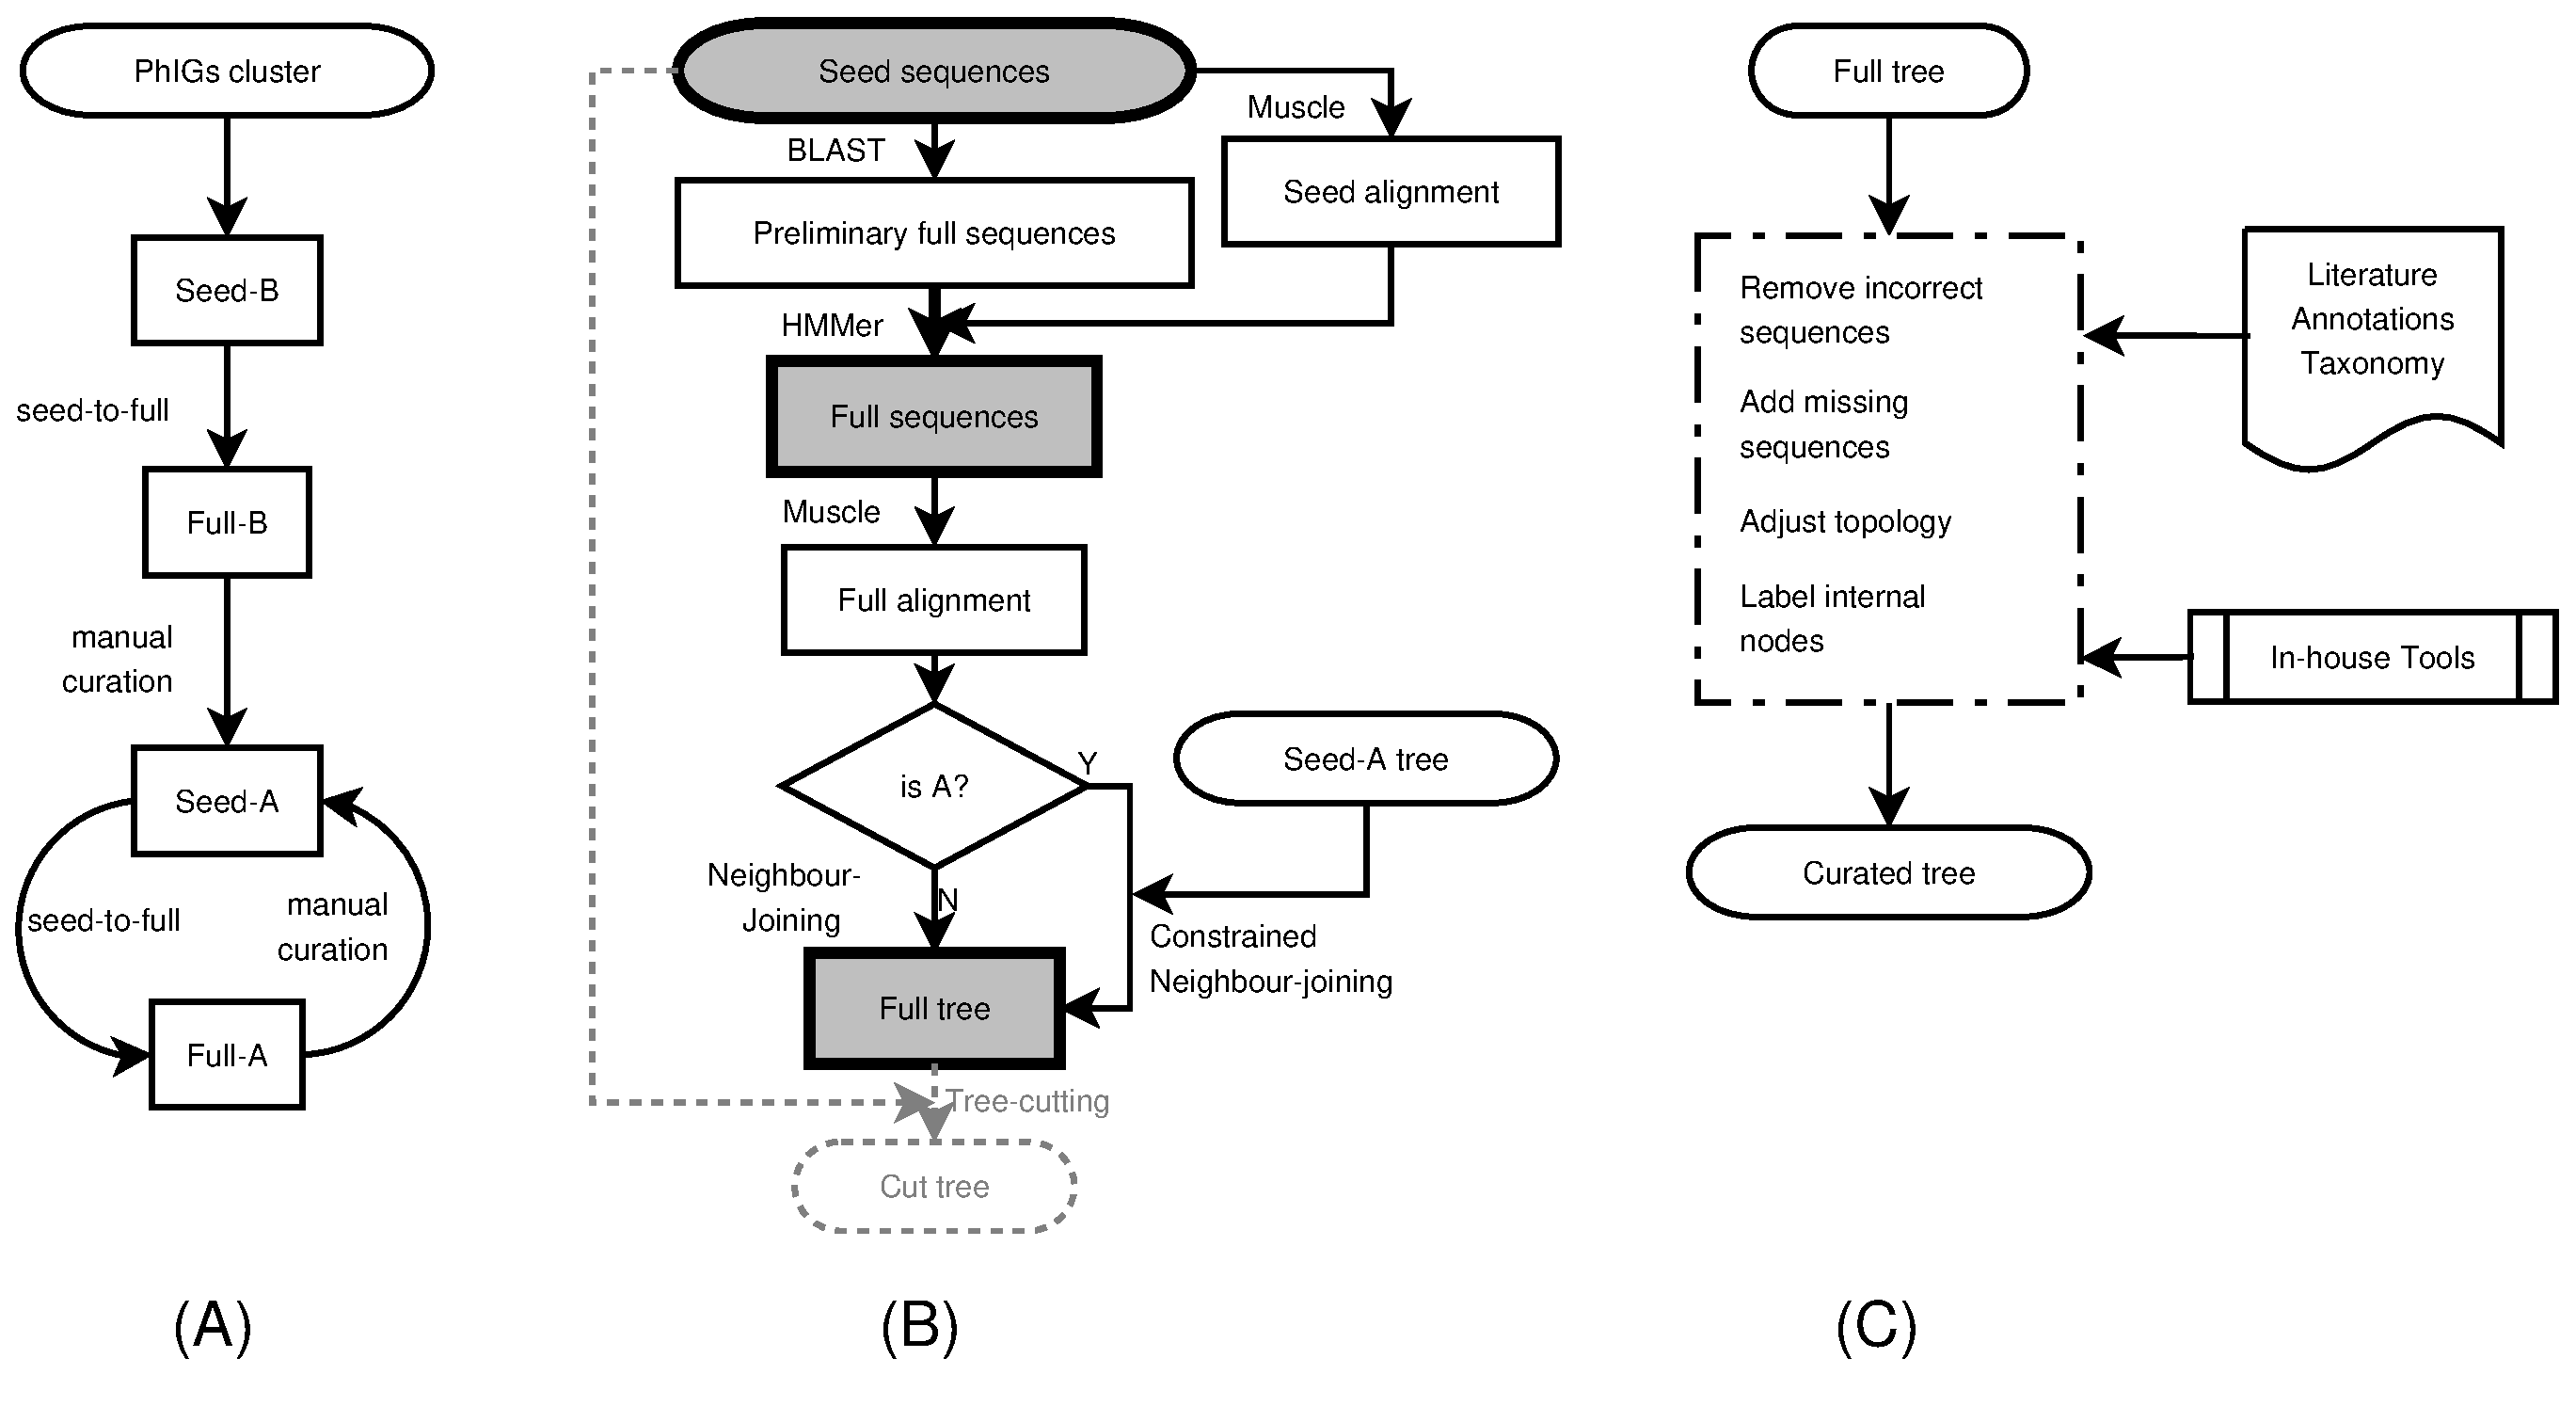
\includegraphics[width=\textwidth]{flowchart}
\caption[Flowchart of TreeFam pipeline]{Flowchart of TreeFam pipeline. (A) Overall strategy. The seed
  families for TreeFam-B are taken from PhIGs clusters. They are expanded by a seed-to-full procedure
  to form full families. Manual curation makes TreeFam-B families become TreeFam-A families, which can
  also be curated further at a later date. (B) The seed-to-full procedure. Dashed lines and gray texts show
  the actions only present in TreeFam-1.x. In the boxes with gray background, details have been changed since
  TreeFam-2. Seed-to-full procedure is used to expand seed sequences to full sequences. Note that
  the complete procedure is only applied when the sequences sets are updated or a whole new genome
  is added to TreeFam. For TreeFam-A families created by curation of a TreeFam-B families,
  the TreeFam-A seed is generated by manual curation, and the full sequences are taken directly
  from the TreeFam-B that was curated. (C) Manual curation. Various published resources and in-house tools
  are utilized in this process.}\label{fig:flowchart}
\end{figure}

\section{Input Data}
\subsection{Sequence data}
TreeFam 2.0 collected protein and coding sequences for 19 fully sequenced species from GenBank~\cite{wheeler05},
SGD~\cite{balakrishnan05}, WormBase~\cite{chen05}, GeneDB~\cite{hertzfowler04} and
Ensembl~\cite{hubbard05} (Table~\ref{tab:species}).
Protein sequences for species that have not
been sequenced were obtained from UniProt~\cite{bairoch05}. Genomic locations and Pfam~\cite{bateman04} domain
structures of genes were also included if available. In this chapter, TreeFam sequence set will be called
TFSEQ\index{TFSEQ} for simplicity.

Of the 19 species, two yeasts and {\it A.thaliana} serve as outgroup species. In a gene tree, genes of outgroup speices
help to reveal ancestral species earlier than the LCA of metazoan animals, and thus indicate
when two groups of animal genes should belong to two TreeFam gene families instead of one.
Outgroups set the boundaries of gene families.

\begin{table}[!hb]
\begin{center}
{\tt
\begin{tabular}{|r|l|l|l|}
\hline
Tax ID & Tax Name & {\it abbr.}	& Common Name\\
\hline
9606	& {\it Homo sapiens}				& HUMAN & Human\\
9598	& {\it Pan troglodytes}				& PANTR & Chimpanzee\\
10090	& {\it Mus musculus}				& MOUSE & Mouse\\
10116	& {\it Rattus norvegicus}			& RAT 	& Rat\\
9615	& {\it Canis familiaris}			& CANFA & Dog\\
9031	& {\it Gallus gallus}				& CHICK & Chicken\\
8364	& {\it Xenopus tropicalis}		& XENTR & Western clawed frog\\
31033	& {\it Fugu rubripes}			& FUGRU & Japanese pufferfish\\
99883	& {\it Tetraodon nigroviridis}	& TETNG & Green puffer\\
7955	& {\it Danio rerio}				& BRARE & Zebrafish\\
7719	& {\it Ciona intestinalis}		& CIOIN & \\
7227	& {\it Drosophila melanogaster}	& DROME & Fruit fly\\
7165	& {\it Anopheles gambiae}		& ANOGA & African malaria mosquito\\
7460	& {\it Apis mellifera}			& APIME & Honeybee\\
6239	& {\it Caenorhabditis elegans}	& CAEEL & \\
6238	& {\it Caenorhabditis briggsae}	& CAEBR & \\
4896	& {\it Schizosaccharomyces pombe}	& SCHPO & Fission yeast\\
4932	& {\it Saccharomyces cerevisiae}	& YEAST & Baker's yeast\\
3702	& {\it Arabidopsis thaliana}		& ARATH & Mouse-ear cress\\
\hline
\end{tabular}
}
\caption[Fully sequenced species that are included in TreeFam-2]
{Fully sequenced species that are included in TreeFam-2. Two yeasts and {\it A.thaliana} serve
as outgroup species that are used to indicate the boundary of a gene family.}~\label{tab:species}
\end{center}
\end{table}

\subsection{Original seeds}
The start point of the entire TreeFam pipelines is the construction of seeds of TreeFam-B families,
which has to be achieved by clustering methods. Fortunately, PhIGs has already done this
in the way we desired. In PhIGs, clusters are inferred to have descended from
a single gene from the last common ancestor of a specified group of species.
Genes are grouped together following the evolutionary relations between species, instead of
sheer similarity scores.
At present, two types of clusters are presented in PhIGs website: one for all vertebrates,
and the other for all metazoan animals. Ideally, a gene cluster of the latter type is exactly equivalent
to a gene family defined in TreeFam, and therefore TreeFam skips the clustering step
and directly uses PhIGs clusters as the original seed sets.

\subsection{Miscellaneous data}
A phylogenetic tree not only presents the history of a gene family. It also
provides the basis for various evolutionary researches, such as studies related to
intron evolution, domain evolution, and shift of gene functions. To help
these studies and to discover the principles behind evolutionary phenomena,
we also integrate several other resources with TreeFam. Since TreeFam-2.0, splicing
information and domain structures of each gene have been available.
Expressional profiles of genes will be provided in TreeFam-3. Phenotypes from
a knockout screen and GO ontology~\cite{ashburner00} categories may also be considered
in future.

\section{Automatic Pipelines}
Pipelines used for constructing TreeFam 2.0 mainly differ from those for 1.x
in two aspects: grouping of PhIGs clusters and use of the competitive method.
As TreeFam paper has already presented detailed procedures used in 1.x series,
we only focus on the 2.0 pipelines in this section.

\subsection{Generating seeds of TreeFam-B families}
In TreeFam release 1.x series, PhIGs clusters that consisted of three or more vertebrate sequences were
directly used as the seeds of TreeFam-B families. However, as PhIGs seemed to apply
a very stringent threshold at clustering stage, it sometimes split a gene family
into several smaller clusters if family members were too divergent.
This has been observed at times in curation processes, and made us
consider clustering PhIGs results when TreeFam 2.0 was planned.

Since TreeFam 2.0, PhIGs clusters are grouped as follows. First, sequences of original clusters
are aligned against TFSEQ by BLAST\footnote{BLAST (Basic Local Alignment Search Tool)
is the most popular alignment program that finds the homologs of one sequence.
It aligns one sequence against each sequence in a sequence set and measures the similarity
by an alignment score. Then BLAST evaluates the significance 
of homology by E-value which is the mathematical expectation of the number of sequences having scores higher than the observed score
when a random sequence is aligned against a random sequence set of the same size.}~\cite{altschul97}
with E-value cutoff $0.01$.
Matched TFSEQs are searched again by HMMER\footnote{HMMER is also a tool for homolog search. It builds an HMM (hidden Markov model)
profile based on a multialignment. It then makes use of the profile to measure how well
a sequence matches the given multialignment. Utilizing a set of sequences, HMMER
is more sensitive and more accurate than BLAST which only performs pairwise alignment.
However, HMMER is much slower than BLAST.}~\cite{eddy98} with E-value cutoff $0.1$.
HMM profiles in this step are built from MUSCLE\footnote{MUSCLE is a multialignment
program like Clustalw. It puts all sequences together and aligns them such that their
homologous regions match with each other. Generally, MUSCLE is much faster and more accurate than
Clustalw~\cite{edgar04}.}~\cite{edgar04} multialignments of original
PhIGs clusters. A relational graph is then constructed from HMMER results. In this graph,
each vertex is an original PhIGs cluster. A weighted edge is added if the HMMER
results of two clusters share some animal genes. More precisely,
given a PhIGs cluster $u$, let $R_u$ be the set of TFSEQ animal genes whose HMMER bit-score
are higher than scores of any outgroup genes matched by sequences in $u$. An edge is added between
two clusters $u$ and $v$ if $R_u\cap R_v\not=\emptyset$. The weight of this
edge is $\frac{|R_u\cap R_v|}{\min\{|R_u|,|R_v|\}}$. After the construction
of this weighted graph, clustering can be achieved by various means
based on graph theory. In TreeFam 2.0, we implemented a heuristic algorithm
revised from Zdobnov {\it et al.}~\cite{zdobnov02}. Like most similar methods, this algorithm tries to find groups
in which edges tend to be saturated~\footnote{As a matter of fact, MCL algorithm~\cite{enright02}
is more sophisticated in this case.}. Finally, grouped PhIGs clusters are
merged to form a larger one, which is regarded as a new cluster in next round.
In theory, this grouping process should be iterated for many times until the results
are stable, but in practice we found that grouping two or more times will
lead to many superfamilies that contain several animal families, seemingly due to the reason that HMMER becomes
insensitive when clusters get larger. Consequently, only one round of
grouping is applied. The results are then used as the seeds of TreeFam-B families.

\subsection{Competitively assigning each sequence to one family}
In TreeFam 1.x, family members were determined by tree cutting algorithm. This algorithm
discarded homologs that are descendants of a different (paralogous) gene in
the last common ancestor of animals. Ideally, such a behaviour is exactly what we desired.
However, due to the tendency of missing distant homologs and the difficulties
in reconstructing long branches, tree cutting malfunctioned at times and resulted
in families that consisted of excessive members. Thus in TreeFam 1.x, one gene
could belong to several or even dozens of families, which by itself was inconsistent and
also caused much trouble in curation. In addition, as multialignments and phylogenetic trees had to be built
before unnecessary sequences were discarded, huge multialignments that contained
over 500 genes were encountered from time to time, which greatly
aggregated computational burden. Consequently, we decided to develop a
better strategy to assign sequences to TreeFam families.

In TreeFam-2.0, homologous sequences are still collected by a combination of BLAST and HMMER:
homologs are first found by BLAST and then refined by HMMER with the profile built from
seed multialignment by MUSCLE. After this step, one sequence
is competitively assigned to one family which gives the
sequence the highest HMMER score; if one family contains several splicing forms of one
gene, only the transcript with the highest HMMER score is retained. Family members
are determined at this time.

To our observations, HMMER usually works quite well if the quality of seeds is
high enough. Most of animal genes, especially vertebrate genes, can be
correctly assigned in this way. However, when seed contains few sequences or
the seed alignment is too poor, HMMER score will be inaccurate and
cause errors. Furthermore, the existence of orphan genes and the
incompleteness of the whole seed set also interfere. Even if a gene does not
belong to any existing TreeFam families, it will still be forcedly assigned
no matter how low the BLAST and HMMER scores are. In the next release of TreeFam,
this problem will be paid more attention.

\subsection{Tracing sequence identifiers for TreeFam-A families}
TreeFam stores curated knowledges in TreeFam-A seed trees. However, with the update
of sequence sets, genes in previous seed trees might be absent in the latest sequence sets when
the identifiers have been changed. In this case, some curation cannot be reserved, and loss of
of information occurs. And continuous loss of information will finally wipe
out all the effort in curation. To slow down this process is very important to a curated
database like TreeFam.

In TreeFam-2.0, a particular pipeline is designed to trace sequence identifiers when they are changed
between releases. The basic idea is to map a new identifier to an old one if~\footnote{These rules
will be changed since TreeFam-3.0.}: (i) the two
sequences come from the same species; (ii) the two are almost identical in matched regions;
and (iii) no other sequence is closer to either of the two sequences. The condition (i) and (ii)
are obvious and can be easily judged. The third condition can be tested by studying the
tree that consists of both unchanged sequences and sequences whose identifiers
are only present in one release, either old or new. In this tree, condition (iii) is satisfied if
a new identifier and an old one share the same parent node. Figure~\ref{fig:exam-traceid} shows
an example where violation of condition (ii) and (iii) occurs.

\begin{figure}[!hb]
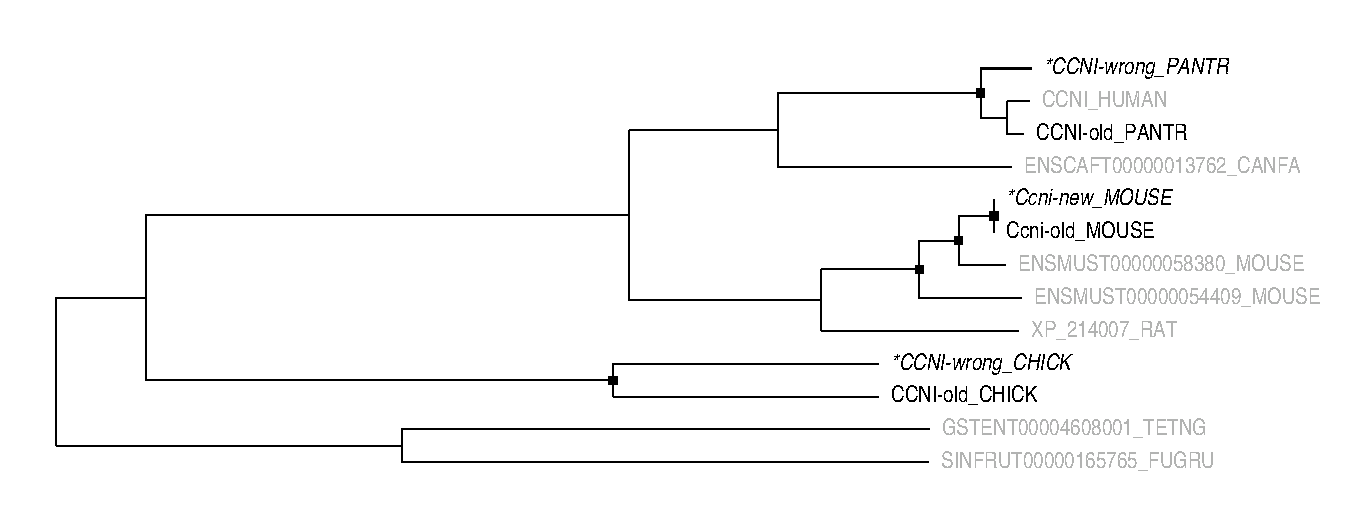
\includegraphics[width=\textwidth]{traceid}
\caption[Example explaining trace-ID procedure]{Example explaining trace-ID procedure. This tree consists of both
unchanged sequences (in gray) and sequences whose identifiers differ between releases (in black).
Sequences only present in the new release are highlighted in slanting font.
Identifier {\tt CCNI-old\_PANTR} shall not be mapped to {\tt *CCNI-wrong\_PANTR}
because {\tt CCNI\_HUMAN} is closer to the former one (violating (iii)).
ID {\tt CCNI-old\_CHICK} cannot be mapped to {\tt *CCNI-wrong\_CHICK} because
they are not close enough (violating (ii)) although they share the same parent node.
Only the two mouse genes can be mapped.
}\label{fig:exam-traceid}
\end{figure}

\subsection{Building trees}
With irrelevant distant homologs discarded in TreeFam-2 families, family trees are much smaller than those in
TreeFam-1.x, which makes it possible to reconstruct trees with more accurate, yet
slower, algorithms such as maximum-likelihood methods. In addition, tree merge algorithm (Chapter~\ref{chap:merge})
is also applied more frequently, and further improves the quality of phylogenetic trees.

In the new TreeFam-B, a full tree is reconstructed, at protein level, by neighbour-joining constrained (Section~\ref{sec:cnj})
by $d_m$ tree, the synonymous-nonsynonymous merged tree. In TreeFam-A, full trees are further required to be constrained by seed trees.
While tree reconstruction at protein level gets more sequences involved,
the use of synonymous tree improves the topologies at lower branches.
In the effort to build even better automatic trees, we also build a `clean tree' that is merged
from four trees including ML protein tree, ML nucleotide tree, NJ synonymous tree and
NJ nonsynonymous tree (Chapter~\ref{chap:merge}). This method really outperforms
all the others both in our benchmark and to our experience in manual curation processes (Chapter~\ref{benchmark}).
